%13.8.03

\chapter{Rechnungen und Details}
\label{sec:fluct_topo}

\section{sc-Gitter mit 18 Nachbarn}
\label{sec:appsc}
Die Vertices des sc-Gitter liegen auf den Ecken von W\"urfeln. Wenn die Vertices des sc-Gitters nicht nur mit ihren sechs n\"achsten Nachbarn, sondern auch mit den zw\"olf Vertices verbunden sind, die eine Fl\"achendiagonale entfernt sind, hat jeder Vertex 18 Nachbarn. W\"urfel um die Vertices m\"ussen also nicht nur \"uber Fl\"achen, sondern auch \"uber gemeinsame Kanten zusammenh\"angen, damit sie die Gitternachbarschaften beschreiben. Andererseits d\"urfen W\"urfel nicht \"uber Ecken verbunden sein. Die mittlere Euler-Charakteristik einer Konfiguration mit diesen Nachbarschaftsverh\"altnissen kann mit der Methode aus Kapitel \ref{sec:mixed} berechnet werden.
\\Die W\"urfel werden mit Wahrscheinlichkeit $p$ besetzt und $\left<\lambda_3\right>=p$. Die $\sigma$'s auf Fl\"achen und Kanten haben den Wert 1. Eine Ecke $c_0$ hat $\sigma(c_0)=0$, es sei denn, alle umliegenden W\"urfel sind besetzt. Wenn immer einer der beiden an eine Fl\"ache $c_2$ angrenzenden W\"urfel besetzt ist, ist $\lambda(c_2)$ Fl\"ache $c_2$ eins und daher $\left<\lambda(c_2)\right>=\left<\lambda_2\right>= 1-(1-p)^2=2p-p^2$. Entsprechend gilt f\"ur die Kanten $\left<\lambda_1\right>  = 1-(1-p)^4 $. Um $\left<\lambda_0\right>$ der Ecken zu bestimmen, werden die alle Besetzungszust\"ande der W\"urfel, die die Ecke umgeben, mit einem Computerprogramm (siehe Anhang \ref{sec:noofcomp}) abgez\"ahlt. Mit $q=1-p$ erh\"alt man
\begin{equation}
  \left< \lambda_0\right> = 8pq^7+32p^2q^6+48p^3q^5+34p^4q^4+16p^5q^3+12p^6q^2+8p^7q+p^8,
\end{equation}
und damit f\"ur das sc-Gitter mit 18 Nachbarn
 \begin{equation}
  \chi_{18-26}^{sc}(p)=p-9p^2+12p^3-3p^4-p^8.
\end{equation}

\section{bcc-Gitter}
\label{sec:appbcc}
Im Kapitel \ref{sec:mixed} wurde f\"ur das bcc-Gitter eine Euler-Charakteristik ausgerechnet, die nur WSZ von Gitternachbarn als benachbart z\"ahlt. Dazu mussten aber WSZ, die sich an Fl\"achen ber\"uhren, die keiner Gitterkante entsprechen, als getrennt aufgefasst werden, solange sie keinen gemeinsamen Gitternachbarn haben. Es gibt auch Zellen, die ohne diesen Umweg Cluster mit den Nachbarschaftsverh\"altnissen des Gitter erzeugen. 
\\Im bcc-Gitter sind die n"achsten Nachbarn eines Gitterpunktes die acht Ecken des umgebenden W"urfels; die Ecken des W\"urfels sind untereinander nicht benachbart (siehe Abb. \ref{fig:bcc}). Daher d\"urfen die Zellen nur mit jenen acht Zellen eine Fl"ache gemeinsam haben, und die Zellen der Vertices auf den Enden einer W"urfelkante d\"urfen sich gegenseitig nur an Kanten ber"uhren. Die vier Zellen auf den Ecken einer Fl\"ache der W\"urfel m"ussen aber die Fl\"ache des W"urfels beinhalten, denn sonst h\"atte die Zelle im Inneren des W"urfels eine Fl"ache mit der Zelle im Inneren des n"achsten W"urfels gemein. Eine m"ogliche Zelle ist in Abbildung \ref{fig:bcc_nonconvex_app} dargestellt. Diese Zelle f"ullt den ganzen Raum, wenn sie um jeden Punkt des bcc-Gitters plaziert wird. Wie immer werden die Zellen mit Wahrscheinlichkeit $q=1-p$ besetzt.
\begin{figure} [htpb]
\centering

\includegraphics{./Fluct_topo-Figs/bcc-zelle}
\caption{Nicht-konvexe Zelle, die angeheftet an jeden Vertex des bcc-Gitters, den Raum f\"ullt; die Struktur der Oberfl"ache ist nur in einem Oktanten gezeigt. Die Zelle hat nur mit acht weiteren Zellen einen ``zweidimensionalen'' Durchschnitt.}
\label{fig:bcc_nonconvex_app}
\end{figure}
Die Euler-Charakteristik wurde mit der Schnittrekursion ausgerechnet. Dazu betrachtet man eine Schar von Ebenen, parallel zu den Grundfl\"achen der W\"urfel. Die Euler-Charakteristik des Schnittes der Ebenen mit den besetzten Zellen \"andert sich dort, wo Ober- und Unterseiten von Zellen in der Ebene liegen. Die Schnitte bestehen aus Quadraten und Kreuzen (siehe Abbildung \ref{fig:bccnonconvexschnitt}). Erstere sind horizontale Schnitte durch die Mitte einer Zelle, letztere die zwei Zellen gemeinsamen Ober- bzw. Unterseiten.
\begin{figure} [htbp]
\centering
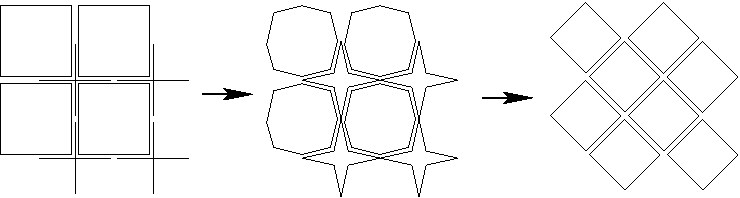
\includegraphics{./Fluct_topo-Figs/bcc-schnitt}
\caption{Schnitt einer Ebene mit den Zellen des bcc-Gitters aus Abb. \ref{fig:bcc_nonconvex_app}: Links ist das Schnittmuster des Schnittes einer Ebene, in der Ober- bzw. Unterseite von Zellen liegen, mit den Zellen des bcc-Gitter gezeigt. Wandert die Ebene weiter, \"andern sich die Muster wie in der Mitte und rechts skizziert. Die Euler-Charakteristik \"andert sich zwischen der mittleren und rechten Situation aber nicht.}
\label{fig:bccnonconvexschnitt}
\end{figure}
Die mittlere Euler-Charakteristik des obigen Schnittes erh"alt man durch wiederholte Schnittrekursion (siehe Abb. \ref{fig:bccschnittzoom}). Die Quadrate sind mit Wahrscheinlichkeit $q$ besetzt, die Kreuze geh\"oren zu zwei Zellen und sind mit Wahrscheinlichkeit $1-p^2$ besetzt. 
\begin{figure}[htbp]
  \centering
  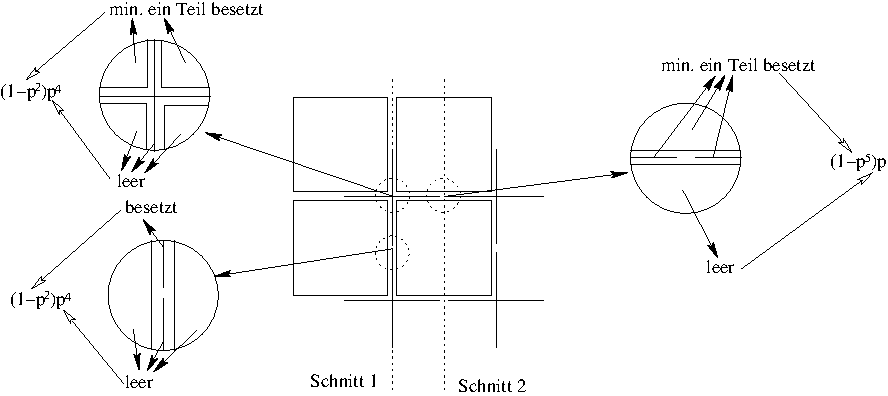
\includegraphics{./Fluct_topo-Figs/bcc-schnittzoom}
  \caption{Wiederholte Schnittrekursion f\"ur das zweidimensionale Schnittmuster. An den beiden gestrichelten Geraden (Schnitt 1 \& 2) \"andert sich die Euler-Charakteristik des Schnittes. Die Punkte, die Beitr\"age zur Euler-Charakteristik der Schnittgeraden liefern, sind in Kreisen vergr\"o"sert dargestellt. Die einzigen Konfigurationen, die Beitr\"age zur Euler-Charakteristik liefern, sind durch ``leer'' und ``besetzt'' beschrieben und ihre Wahrschneinlichkeit sind angegeben (vergleiche Gleichung (\ref{eq:bccschnitt})). Die \"ubrigen Terme aus Gleichung (\ref{eq:bccschnitt}) entstehen durch leicht verschobene Schnitte und lassen sich analog ablesen.  }
  \label{fig:bccschnittzoom}
\end{figure}
Man betrachtet Schnittgeraden parallel zu einer der Quadratseiten. Die Euler-Charakteristik des Schnittes einer solchen Geraden mit dem zweidimensionalen Schnittmuster kann sich dort \"andern, wo die Gerade zwischen Quadraten oder Kreuzen liegt. Die verschiedenen Beitr\"age sind in Abbildung \ref{fig:bccschnittzoom} dargestellt und man erh\"alt 
\begin{equation}
\label{eq:bccschnitt}
  \begin{split}
    \chi_2(q) &=\chi_1^{(1)}-\chi_1^{(1)+}+\chi_1^{(2)}-\chi_1^{(2)+}\\
          &=\frac{1}{2} \left[ 2(1-p^2)p^4 - (1-p^3)p \right] \\
         &  + \frac{1}{2} \left[ (1-p^5)p - (1-p^3)p \right] \\
          & =  \frac{1}{2} \left[ -3p^6+4p^4-p \right].
\end{split}
\end{equation}
Zu den beiden Schnitten aus Abb. \ref{fig:bccschnittzoom} tragen zwei Reihen von Zellen bei, daher der Faktor $\frac{1}{2}$.
Die Euler-Charakteristik jedes anderen Schnittes der Ebene mit den Zellen ist die des Quadratgitters mit \"ubern\"achsten Nachbarn (siehe Abbildung \ref{fig:bccnonconvexschnitt}, rechts):
\begin{equation}
   \chi_2^+(q) =  -p^4+2p^2-p.
\end{equation}
Pro Zellenschicht gibt es zwei Schnitte dieser Art und die Euler-Charakteristik des bcc-Gitters, eingeteilt in diese Zellen, ist damit
        \begin{equation}
          \chi^{bcc}_{8-26}(p)=\bar{\chi}(q)=-3p^6+6p^4-4p^2+p.
        \end{equation}
Jede Zelle h\"angt mit acht Zellen \"uber eine Fl\"ache zusammen und mit 18 weiteren \"uber Ecken und Kanten zusammen.


\section{Diamantgitter}
\label{sec:appdiamant}
\subsection{Konvexe Zellen}
\label{sec:appdiamantconvex}
Da das Diamantgitter ein fcc-Gitter mit zweiatomiger Basis ist, bietet es sich an, als Zelle um die Vertices eine senkrecht zur Basisachse halbierte Wigner-Seitz-Zelle (WSZ) des fcc-Gitters zu nehmen (siehe Abb. \ref{fig:fcc_half}). Diese halbierten Zellen haben mehr Fl\"achen, als ein Vertex Nachbarn hat, und die Zusammenhangsverh\"altnisse des Diamantgitters werden durch Wahl der $\sigma$-Variablen erzwungen (siehe Kapitel \ref{sec:mixedbcc}).   
\begin{figure}[htbp] 
  \centering
  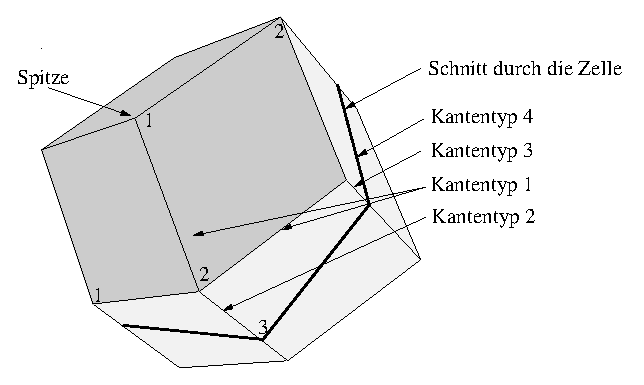
\includegraphics{./Fluct_topo-Figs/fcc_half}
  \caption{Eine WSZ des fcc-Gitter. Die dicke Linie soll die Halbierung der Zelle andeuten. Jede H\"alfte ist Zelle eines Vertex des Diamantgitters. Die Zahlen an den Ecken beziehen sich auf die verschiedenen Vertextypen; auch die verschiedenen Kantentypen sind bezeichnet (siehe Text). Die drei dunkelgrauen Fl\"achen und die neuentstandenen Schnittfl\"ache entsprechen den Gitterkanten des Diamantgitters.}
  \label{fig:fcc_half}
\end{figure}
\\Die halbierten Zellen werden mit Wahrscheinlichkeit $p=1-q$ besetzt und $\left<\lambda_3\right>=p$. Die oberen Rauten, in Abb. \ref{fig:fcc_half} dunkelgrau gezeichnet, und die Schnittfl\"ache entsprechen Gitternachbarschaften und haben $\sigma^{nn}=1$. Zellen, die sich an anderen Fl\"achen ber\"uhren, sollen nur zusammenh\"angen, wenn sie einen gemeinsamen n\"achsten Nachbarn haben. F\"ur diese Fl\"achen ist $\sigma^{nnn}$ nur dann 1, wenn ihr gemeinsamer n\"achster Nachbar besetzt ist. F\"ur die Fl\"achen, die n\"achsten Nachbarn entsprechen, gilt $\left< \lambda_2^{nn}\right>=1-q^2$, f\"ur alle \"ubrigen Fl\"achen 
\begin{equation}
   \left< \lambda_2^{nnn}\right> =p(1-q^2)+q(2p^2+2pq).
\end{equation} 
Die $\sigma$'s aller Kanten und Ecken sind 0, sofern nicht alle umgebenden Zellen besetzt sind und die Fl\"achen zwischen ihnen $\sigma=1$ haben. Eine Zelle hat vier verschiedene Typen von Kanten, die unterschiedlich behandelt werden m\"ussen (siehe Abb. \ref{fig:fcc_half}). Zum ersten Typ geh\"oren die drei Kanten auf der Spitze der Zelle. Sie entsprechen den Kanten auf dem oberen Rand anderer Zellen. Daher geh\"oren die Kanten auf der Spitze und auf dem oberen Rand der Zellen zum Typ 1. Die Kanten, die parallel zur Basisachse sind, kommen in zwei unterschiedlichen L\"angen vor und bilden die Typen 2 und 3. Die Kanten entlang des Schnittes seien Typ 4.
\\Eine Kante des ersten Typs ist in drei Zellen enthalten. Sie ist eine Kante auf der Spitze einer Zelle $z1$ und eine Kante auf dem oberen Rand der beiden anderen Zellen $z2$ und $z3$. Die Zelle $z1$ ist gemeinsamer n\"achster Nachbar der Zellen $z2$ und $z3$. Die Kante ist mindestens einmal vorhanden, wenn eine der Zellen besetzt ist. Nur wenn die Zelle $z1$ unbesetzt ist, und die Zellen $z2$ und $z3$ beide besetzt sind, ist $\lambda_1^{T1}=2$.
\begin{equation}
\left<\lambda_1^{T1}\right>=(1-q^3)+qp^2
\end{equation}
Zur Veranschaulichung f\"uhren wir f\"ur die verbleibenden Typen je einen Graphen ein, dessen Vertices den die Kante umgebenden Zellen entsprechen. Die Verbindungen zwischen den Vertices entsprechen den Fl\"achen zwischen den Zellen (siehe Abb. \ref{fig:diagraph}). Vertices sind mit Wahrscheinlichkeit $p$ besetzt, die Verbindungen sind, abh\"angig von anderen Zellen, mit bestimmten Wahrscheinlichkeiten pr\"asent. 
\begin{figure}[htbp] 
  \centering
  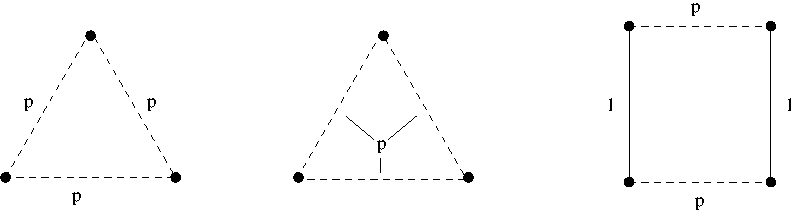
\includegraphics{./Fluct_topo-Figs/diagraph}
  \caption{Links der Graph des Kantentyps 2: Die drei Vertices und Verbindungen existieren unabh\"angig voneinander mit Wahrscheinlichkeit $p$. In der Mitte der Graph des Kantentyps 3: Die drei Vertices sind unabh\"angig voneinander jeweils mit Wahrscheinlichkeit $p$ besetzt; mit Wahrscheinlichkeit $p$ sind alle Vertices verbunden. Rechts der Graph des Kantentyps 4: Die Vertices sind mit Wahrscheinlichkeit $p$ besetzt, senkrechte Verbindungen existieren immer und waagerechte mit Wahrscheinlichkeit $p$.}
  \label{fig:diagraph}
\end{figure}
Kanten des Typs 2 sind die langen Kanten parallel zur Basisachse. Um eine solche Kante sind drei Zellen angeordnet, und je zwei der Zellen haben einen gemeinsamen Gitternachbarn. D.h. Vertices und Kanten des entsprechenden Graphen sind unabh\"angig voneinander mit Wahrscheinlichkeit $p$ vorhanden (linker Graph in Abb. \ref{fig:diagraph}). Kanten des Typs 3 sind die kurzen Kanten parallel zur Basisachse. Die Kante ist Teil von drei Zellen, die alle den gleichen gemeinsamen Gitternachbarn haben. Alle Verbindungen des Graphens sind daher mit Wahrscheinlichkeit $p$ vorhanden (mittlerer Graph in Abb. \ref{fig:diagraph}). Kanten des Typs 4 sind die durch die Halbierung der fcc-WSZ entstandenen Schnittkanten. Eine Kante des Typs 4 wird von vier Zellen umgeben, von denen die Zellen, die zu einer fcc-WSZ geh\"oren, Gitternachbarn sind. Die zwei Zellen auf der einen und auf der anderen Seite der Schnittebene haben je einen gemeinsamen Gitternachbarn (rechter Graph in Abb. \ref{fig:diagraph}). $\lambda_1$ berechnet sich aus den Besetzungszust\"anden der Zellen und Fl\"achen (Vertices und Kanten dieser Graphen). Durch Abz\"ahlen aller Konfigurationen erh\"alt man:
\begin{eqnarray}
\left<\lambda_1^{T2}\right> & = &\begin{split} 
 & p^3(1-q^3)+3p^2q(p^3+4p^2q+3pq^3)\\  & +3pq^2(2p^3+5p^2q+3pq^2)+q^3(3p^3+6p^2q+3pq^2)
\end{split}\\
\left<\lambda_2^{T3}\right> & = & p(1-q^3)+q(3p^3+6p^2q+3pq^2)\\
 \left<\lambda_2^{T4}\right> & = &\begin{split}&
  p^2(1-q^4)+2pq(p^4+6p^3q+9p^2q^2+4pq^3)\\ & +q^2(2p^4+8p^3q+10p^2q^2+4pq^3)
\end{split}
\end{eqnarray}
Es gibt 3 Typen von Vertices, die unterschiedlich zur Euler-Charakteristik beitragen (siehe Abb. \ref{fig:fcc_half}). Die Spitze einer Zelle ist gleichzeitig eine tiefliegende Ecke auf dem oberen Rand von drei anderen Zellen. Diese Vertices seien Typ 1. Die h\"oherliegenden Vertices auf dem oberen Rand seien Typ 2 und die durch die Halbierung der fcc-WSZ entstandenen Vertices Typ 3. Die Umgebungen der Vertices lassen sich wiederum  durch Graphen anschaulich darstellen (siehe Abb. \ref{fig:vertexgraph}). Jeder Vertex des Graphens entspricht einer Zelle und jede Verbindung einer Fl\"ache. Die Fl\"achen des Graphens entsprechen den Kanten, die die Ecke umgeben.
\begin{figure}[htbp]
  \centering
  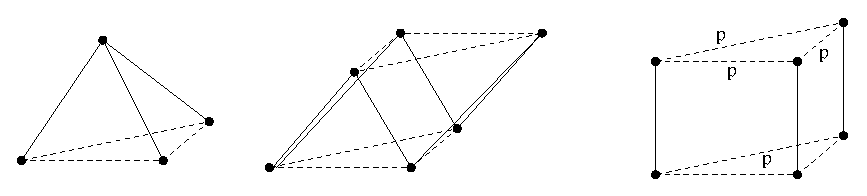
\includegraphics{./Fluct_topo-Figs/vertexgraph}
  \caption{Die Graphen der drei Vertextypen: Der Graph von Typ 1 (links) besteht aus den Vertices eines Tetraedes, dessen Spitze mit allen anderen Vertices verbunden sind. Die Vertices der Grundfl\"ache sind untereinander nur verbunden, wenn die Spitze besetzt ist. In der Mitte ist der Graph von Vertextyp 2 dargestellt. Er besteht aus einer Schleife von sechs Vertices. \"Ubern\"achste Vertices sind verbunden, wenn der Vertex zwischen ihnen besetzt ist. Der Graph von Vertextyp 3 (rechts) ist ein Prisma dreieckiger Grundfl\"ache. Senkrechte Verbindungen existieren immer, die der Kopffl\"ache jeweils mit Wahrscheinlichkeit $p$ und die der Fu"sfl\"ache alle mit Wahrscheinlichkeit $p$.}
  \label{fig:vertexgraph}
\end{figure}
\\Vertextyp 1 wird von vier Zellen umgeben, von denen eine der gemeinsame n\"achste Nachbar der drei anderen ist. Diese Zelle ist die Spitze des Tetraeders in Abb. \ref{fig:vertexgraph}. Sobald der Vertex auf der Spitze des Tetraeders besetzt ist, sind die Verbindungen in der Grundfl\"ache vorhanden, und es kann nur eine Komponente entstehen, die keine L\"ocher hat. Wenn immer die Spitze besetzt ist, ist $\lambda=1$. Ist die Spitze unbesetzt, sind die drei verbleibenden Vertices isoliert. Den isolierten Vertices entsprechen isolierte Zellen, die je 1 zu $\lambda_0$ beitragen, und man erh\"alt
\begin{equation}
\left<\lambda_0^{T1}\right>=p+q(3p^3+6p^2q+3pq^2).
\end{equation}
Um einen Vertex vom Typ 2 sind zweimal drei Zellen angeordnet, die keine Gitternachbarn sind. Je ein Vertex der einen Dreiergruppe ist gemeinsamer Gitternachbar zweier Vertices der anderen Dreiergruppe. Der Graph von Typ 2 besteht daher aus einem Zyklus von sechs Vertices, indem Verbindungen von Vertex $i-1$ zu Vertex $i+1$ hinzugef\"ugt werden, wenn Vertex $i$ besetzt ist. Diese Anordnung wird im Computerprogramm (siehe Kapitel \ref{sec:noofcomp}) implementiert. Das Ergebnis ist:
\begin{equation}
\left<\lambda_0^{T2}\right>=6pq^5+24p^2q^4+36p^3q^3+24p^4q^2+6p^5q+p^6.
\end{equation}
Ein Vertex von Typ 3 liegt auf dem Schnitt, der die fcc-Zelle halbiert. Er ist von drei Paaren von Vertices umgeben, die zu einer fcc-WSZ geh\"oren und daher Gitternachbarn sind. Die drei Zellen auf der einen Seite des Schnittes haben einen gemeinsamen Gitternachbarn, von denen auf der anderen Seite haben je zwei einen gemeinsamen Gitternachbarn. Der Graph von Vertextyp 3 ist ein Prisma dreieckiger Grundfl\"ache, dessen senkrechte Verbindungen immer, die im oberen Dreieck jeweils mit Wahrscheinlichkeit $p$ und die im unteren Dreieck alle mit Wahrscheinlichkeit $p$ existieren. Die Konfigurationen wurden mit dem Computerprogramm abgez\"ahlt und man erh\"alt 
\begin{equation}
\begin{split}
\left<\lambda_0^{T3}\right>= & 6q^9p+51q^8p^2+186q^7p^3+379q^6p^4+468q^5p^5 \\ & +355q^4p^6+162p^7q^3+45q^2p^8+10qp^9+p^{10}
\end{split}
\end{equation}
Die Anzahl der Fl\"achen, Kanten und Ecken pro Zelle ist schnell bestimmt und alternierendes Aufsummieren liefert
\begin{equation}
\chi_{4-19}^{Diamant}(p)=p(1-p)(p^8+p^7+p^6+p^5-4p^4+2p^3-p^2-p+1).
\end{equation}

\subsection {Geteilte primitive Einheitszellen}
\label{sec:appdiamantnonconvex}
Um der Topologie des Diamantgitters mit seinen vier n"achsten 
Nachbarn Rechnung zu tragen, ohne die Zusammenhangsverh\"altnisse ``k\"unstlich'' zu erzwingen, ist eine Zelle n"otig, die nur mit 
den Zellen der vier Gitternachbarn eine Fl"ache gemeinsam hat. 
Hierzu betrachtet man die primitive Einheitszelle des fcc-Gitters. 
Dieses Parallelepiped f"ullt den gesamten Raum, wenn es an jeden 
Gitterpunkt des fcc-Gitters angeheftet wird. Wird das Diamantgitter 
als fcc-Gitter mit zweiatomiger Basis auf diese Weise zerlegt, 
liegt ein Gitterpunkt an einem spitzen Ende des Parallelepiped, der andere 
innerhalb. Verschiebt man das Parallelepiped  entlang der durch die Basis 
ausgezeichneten Richtung soweit, dass beide Basisatome symmetrisch in 
in ihm liegen, kann man das Parallelepiped derart teilen, dass in jeder H\"alfte ein Vertex des Diamantgitters liegt (siehe Abb. \ref{fig:appdiazelle}). Die Teilung muss so 
erfolgen, dass drei der Fl"achen des Parallelepipids zu einer 
Zelle, die "ubrigen zur anderen Zelle geh"oren. Um die 
Berechnung der Euler-Charakteristik zu erleichtern, ist es zweckm\"a"sig, das 
Gitter derart zu deformieren, dass aus dem Parallelepiped ein 
W"urfel wird. Das "andert nicht die Topologie, sondern nur die 
Abst"ande der Gitterpunkte.
\begin{figure}[htbp]
\begin{center}
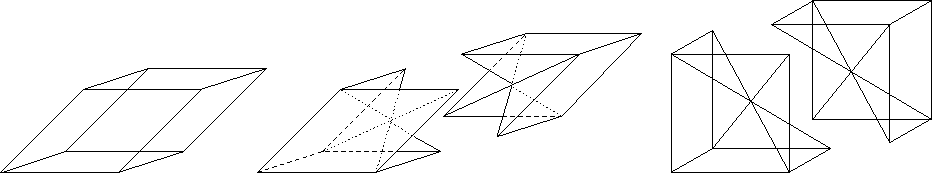
\includegraphics{./Fluct_topo-Figs/geteilte_zelle}
\caption{Das Parallelepiped und seine Teilung; Teilung des zu einem W"urfel deformierten Parallelepipeds}
\label{fig:appdiazelle}
\end{center}
\end{figure}
\\Die Fl\"ache, die durch die Teilung entsteht, ist nicht eben. Der Beitrag der Fl\"ache, ohne die \"au"seren W\"urfelkanten, zur Euler-Charakteristik ist aber wie bei einer ebenen Fl\"achen ohne Rand gleich $1$. Besetzt man die Zellen mit Wahrscheinlichkeit $q=1-p$, so ist eine Fl\"ache, ob eben oder nicht, mit Wahrscheinlichkeit $1-p^2$ vorhanden. Jede W\"urfelkante geh\"ort zu sechs Zellen und ist daher mit Wahrscheinlichkeit $1-p^6$ Teil einer Figur aus mit Wahrscheinlichkeit $q$ besetzten Zellen. Eine Ecke eines W\"urfels ist in 14 Zellen enthalten und daher mit Wahrscheinlichkeit $1-p^{14}$ vorhanden. Pro Zelle gibt es vier Fl\"achen, die jeweils zu zwei Zellen geh\"oren, neun W\"urfelkanten, die jeweils zu sechs Zellen geh\"oren, und sieben W\"urfelecken, die jeweils zu 14 Zellen geh\"oren. F\"ur die Euler-Charakteristik erh\"alt man
\begin{equation}
  \begin{split}
  \chi^{diamant}_{4-47}(p) & = \bar{\chi}(q)=\frac{1}{2}(1-p^{14})-\frac{3}{2}(1-p^6)+2(1-p^2)-(1-p) \\
  &= -\frac{p^{14}}{2}+\frac{3p^6}{2}-2p^2+p
\end{split}
\end{equation}
   Die Zellen haben mit nur vier anderen Zellen eine gemeinsame 
   Fl"ache und diese Fl\"achen entsprechen den Gitternachbarschaften 
   im Diamantgitter. Allerdings haben diese Zellen sehr viele 
   Nachbarn, mit denen sie "uber Kanten oder Ecken zusammenh"angen. Zur Ermittlung der Zahl der Nachbarn einer Zelle betrachtet man 
   den Einheitsw"urfel, bestehend aus zwei Zellen, und alle 26 
   umliegenden W"urfel. Das sind zusammen 54 Zellen, von denen nur
   sechs nicht mit der betrachteten Zelle benachbart sind. Weiter 
   entfernte Zellen sind nicht mit der Zelle benachbart. Eine Zelle hat also mit $47$ anderen Zellen einen nichtleeren Durchschnitt.
   

\section{fcc-Gitter}
\label{sec:appfcc}
\subsection{Wigner-Seitz-Zelle}
Die Wigner-Seitz-Zelle (WSZ) des fcc-Gitters ist ein rhombisches Dodekaeder. Die WSZ hat zw\"olf Fl\"achen, 24 Kanten und 14 Ecken. 
Wir besetzen die WSZ eines fcc-Gitters mit Wahrscheinlichkeit $q=1-p$. Eine Fl\"ache ist immer dann belegt, wenn eine der beiden WSZ, zu denen diese Fl\"ache geh\"ort, besetzt ist, und daher mit Wahrscheinlichkeit $1-p^2$ vorhanden. Jede Kante ist Teil von drei WSZ und mit Wahrscheinlichkeit $1-p^3$ vorhanden. Von den 14 Ecken geh\"oren sechs Ecken zu sechs WSZ und die \"ubrigen acht Ecken zu vier WSZ. Erstere sind mit Wahrscheinlichkeit $1-p^6$ belegt, letztere mit Wahrscheinlichkeit $1-p^4$. F\"ur die Euler-Charakteristik erh\"alt man damit
\begin{equation}
  \begin{split}
  \chi(p)= & \bar{\chi}(q)=(1-p^6)+2(1-p^4)-8(1-p^3)+6(1-p^2)-(1-p)\\
  &=p-6p^2+8p^3-2p^4-p^6.
\end{split}
\end{equation}

\subsection{Prismen als Zellen des fcc-Gitters}
Das fcc-Gitter ist ein Stapel gegeneinander verschobener Quadratgitter (siehe Kapitel \ref{sec:schrfcc}). Die Vertices einer Ebene liegen in der Mitte der Plaketten der dar\"uber und darunter liegenden Ebenen. Die Nachbarn eines Vertex des fcc-Gitters sind die Nachbarn im Quadratgitter seiner Ebene, sowie die Vertices auf dem Rand der Plaketten "uber und unter ihm. Legt man um die Vertices raumf\"ullende Prismen quadratischer Grundfl\"ache, so haben diese Prismen nur mit Gitternachbarn eine Fl\"ache gemein. In ihrer Ebene sind das die vier Seitenfl\"achen, in den Ebenen darunter und dar\"uber \"uberlappen die Prismen an den Kopf- bzw. Fu"sfl\"achen mit je vier Prismen. Im Unterschied zu WSZ haben die Prismen aber nur vier weitere Nachbarn, mit denen sie \"uber die senkrechten Kanten der Prismen zusammenh\"angen. Die Euler-Charakteristik wurde mit der Schnittrekursion berechnet. Die Euler-Charakteristik des Schnittes einer Ebene mit den besetzten Zellen \"andert sich nur zwischen zwei Prismenebenen. Die Euler-Charakteristik dieses Schnitts wird durch wiederholte Schnittrekursion bestimmt. Die Terme, die zur Euler-Charakteristik beitragen, sind in Abbildung \ref{fig:fcc_quader} skizziert. Jeder andere Schnitt hat die mittlere Euler-Charakteristik des Quadratgitters mit \"ubern\"achsten Nachbarn. F\"ur die Euler-Charakteristik des fcc-Gitters erh\"alt man 
\begin{equation}
\begin{split}
\chi^{fcc}_{12-16}(p)=\bar{\chi}(q) & = \bar{\chi}_{2}(q)-\bar{\chi}^{sq}(q) \\
       & =  2\left[(1-p^2)p^3+(1-p)p^3 - 
       2qp^2\right]-\left[ -p^4+2p^2-p \right]\\
       & = -2p^5-p^4+8p^3-6p^2+p
\end{split}
\end{equation}

\begin{figure}[tpb]
\centering
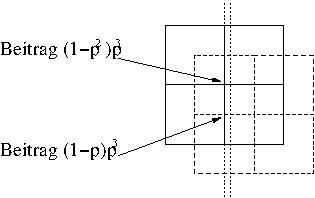
\includegraphics{./Fluct_topo-Figs/fcc-qu-schnitt}
\caption{Schnitt zwischen zwei Schichten von Prismen. Die Wahrscheinlichkeiten der einzigen beiden Konfigurationen, die zur Euler-Charakteristik beitragen, sind angegeben. Durchgezogene Quadrate sind Fu"sfl\"achen der einen Prismenschicht, die gestrichtelten Quadrate die Kopffl\"achen der anderen Schicht. Die Prismen sind jeweils mit Wahrscheinlichkeit $q=1-p$ besetzt. }
\label{fig:fcc_quader}
\end{figure}


\section{Bond-site-Perkolation}
\label{sec:appbond-site}
Um die Euler-Charakteristik eines bond-site-Perkolationsprozesses auszurechnen, m\"ussen (siehe Kapitel \ref{sec:bond-site}) die Erwartungswerte $\left< \lambda_i\right>$ der unterschiedlichen Zellen berechnet werden. 
\subsection{Dreiecksgitter}
Das duale Gitter des Dreiecksgitters ist das Sechseckgitter. Die Sechsecke sind mit Wahrscheinlichkeit $p_s$ besetzt und f\"ur Sechsecke gilt $\left<\lambda_2\right>_{p_s,p_b}=p_s$. Es gibt drei Kanten pro Sechseck und jede Kante ist mit Wahrscheinlichkeit $p_b$ besetzt. Daher ist $\left<\lambda_1\right>_{p_s,p_b}=(1-(1-p_s)^2)p_b-2p_s(1-p_b)=2p_s-p_bp_s^2$. Jede Ecke ist von drei Sechsecken und drei Kanten umgeben. Diese Anordnung ist einfach zu implementieren (siehe Kapitel \ref{sec:noofcomp}), und das Programm liefert
\begin{equation}   
\left< \lambda_0 \right>_{p_s,p_b} = p_s^3p_b^3-3p_s^2p_b+3p_s.
\end{equation}
F\"ur die Euler-Charakteristik der bond-site-Perkolation auf dem Dreiecksgitter erh\"alt man 
\begin{equation}
  \begin{split} \chi^{tr}(p_s,p_b)& = \left<\lambda_2\right>_{p_s,p_b}-3\left<\lambda_1\right>_{p_s,p_b}+3\left< \lambda_0 \right>_{p_s,p_b}\\
& = p_s-3p_bp_s^2+2p_b^3p_s^3.
\end{split}
\end{equation}

\subsection{fcc-Gitter}
Um die Euler-Charakteristik des fcc-Gitters zu bestimmen, besetzen wir die WSZ des Gitters mit Wahrscheinlichkeit $p_s$. Zwei besetzte WSZ sind \"uber eine gemeinsame Fl\"ache mit Wahrscheinlichkeit $p_b$ verbunden. Aus Kapitel \ref{sec:bond-site} haben wir $\left<\lambda_3\right>_{p_s,p_b}=p_s$ und $\left<\lambda_2\right>_{p_s,p_b}=2p_s-p_bp_s^2$. Eine Kante der WSZ geh\"ort zu drei Zellen und $\left<\lambda_1\right>_{p_s,p_b}$ ist daher gleich $\left< \lambda_0^{tr} \right>_{p_s,p_b}$ des Dreiecksgitters. Insgesamt hat eine WSZ 24 Kanten und damit acht pro Zelle. 
\\Acht der 14 Ecken der WSZ geh\"oren zu vier WSZ, deren Mittelpunkte auf einem Tetraeder angeordnet sind. Die Fl\"achen zwischen den WSZ entsprechen den Kanten des Tetraeders. Die vier Zellen, sechs Fl\"achen und vier Kanten, die eine solche Ecke umgeben, m\"ussen im Quelltext des Programms definiert werden. Abz\"ahlen aller Konfigurationen liefert:
\begin{equation}
\left<\lambda_0^1\right>_{p_s,p_b} = 3p_b^4p_s^4-6p_b^5p_s^4+2p_b^6p_s^4+4p_b^3p_s^3-6p_bp_s^2+4p_s.
\end{equation}
Die anderen sechs Ecken der WSZ geh\"oren zu sechs WSZ. Die Mittelpunkte der sechs Zellen liegen auf den Ecken eines Oktaeders. Die zw\"olf Kanten des Oktateders entsprechen den Fl\"achen zwischen den Zellen, und die acht Fl\"achen entsprechen den Kanten, die die Ecke umgeben. Das Programm aus Kapitel \ref{sec:noofcomp} liefert
\begin{equation}
\left<\lambda_0^2\right>_{p_s,p_b} =6p_s-12p_bp_s^2+8p_b^3p_s^3-p_b^{12}p_s^6.
\end{equation}
Die Euler-Charakteristik der bond-site-Perkolation auf dem fcc-Gitter ist damit: 
\begin{equation}
  \begin{split} \chi^{fcc}(p_s,p_b)& = -\left<\lambda_3\right>_{p_s,p_b}+6\left<\lambda_2\right>_{p_s,p_b}-8\left< \lambda_1 \right>_{p_s,p_b}+2\left<\lambda_0^1\right>_{p_s,p_b}+\left<\lambda_0^2\right>_{p_s,p_b}\\
& =p_s-6p_bp_s^2+8p_b^3p_s^3-2p_b^6p_s^4-p_b^{12}p_s^6.
\end{split}
\end{equation}


